\chapter{Fudge factors}
\label{ch:ffs}
\epigraph{\emph{“Champions keep playing until they get it right.”}}{Billie Jean King}




The \ac{FF} method has been applied to photons in \ac{ATLAS} as simple shifts of the distributions. In this chapter, a detailed explanation of the calculation is shown, with the addition of improvements derived for this type of corrections.







\section{Calculation}

\acp{FF} are computed in a series of steps that starts by preparing the input datasets up to the systematic uncertainties calculation. In the first step, histograms of all the \acp{SSV} are created and then smoothed, which are then used to perform the actual optimisation of the \acp{FF}. This process is repeated for different isolation and identification selection requirements, in order to compute the systematic uncertainties. In the following a step by step description of the process is described.

The calculation is performed separately for the two considered samples: \ac{RZ} for photons with \(7\leq\pt\leq 50~\gev\) and \ac{SP} for photons with \(\pt> 50~\gev\). Since \acp{SS} distributions vary as a function of \pt and \abseta, the computation is done in bins of these mentioned variables:
\begin{gather}
    \ptgam:
    \begin{cases}
        \text{\ac{RZ}}: [7, 15, 20, 30, 50] ~\gev\\
        \text{\ac{SP}}: (50, 60, 80, 100, 150, 300, 600, \infty] ~\gev\\
    \end{cases}\\
    \abseta: [0, 0.6, 0.8, 1.15, 1.37, 1.52, 1.81, 2.01, 2.37].
\end{gather}
Furthermore, as mentioned in \Sect{\ref{sec:pid_ss:ss}}, there are variables very sensitive to the conversion status of the photons, that is, whether if the photons are converted or unconverted. For this reason, the calculation is done separately for converted and unconverted photons. A total of nine variables are corrected using this method: \eratio, \fside, \reta, \rphi, \rhad, \rhado, \wone, \weta and \wstot; as they are the ones in which the largest discrpancies are seen between data and \ac{MC}.

For each mentioned \ac{SSV}, histograms of \ac{MC} and data of 100 bins are created. The choice of the binning is done based on having sufficient statistics at each bin and also to capture all the features of the variables.

After that, each histogram is smoothed using the \ac{KDE} tool from TMVA~\cite{TMVA}. The \ac{KDE} method consists of estimating the shape of a \ac{pdf} by the sum over smeared events. The \ac{pdf} \(p(x)\) of a variable \(x\) is
\begin{equation}
	p(x) = \frac{1}{N}\sum_{i=1}^{N} K_h(x-x_i)
\end{equation}
where \(N\) is the number of events, \(K_h(t) = K(t/h)/h\) is the kernel function, and \(h\) is the bandwidth of the kernel. The basic idea is that each event is considered as a Dirac-\(\delta\)-function, which are replaced by a Kernel function (Gaussian) and finally they are summed altogether to form the final \ac{PDF}. The \ac{KDE} smoothing can be applied in two forms: non-adaptive \ac{KDE} or adaptive \ac{KDE}, as seen in FIGURE. In the former, the bandwidth is constant for the entire sample \(h_{NA}\), while in the latter, it uses the value from non-adaptive \ac{KDE}, but it varies as a function of \(p(x)\) as
\begin{equation}
	h_A = \frac{h_{NA}}{\sqrt{p(x)}}
\end{equation}
Adaptive \ac{KDE} improves the shape of the estimated \ac{pdf} in regions of low statistics, however, in high statistics regions it can give rise to "over-smoothing". The degree of smoothing is tuned by multiplying the bandwidth \(h\) by fine factors. 
These fine factors are user-defined parameter which are tuned to allow the \ac{pdf} to retain the important features of the \ac{SS} but to also avoid statistical fluctuations. Higher values indicate broader Kernel functions and therefore de \ac{pdf} catches less statistical fluctuations.
Examples of the smoothing procedure applied to \(R_{\eta}\) are shown in FIGURE for cases in which original histograms have low and high statistics.




Once the data and \ac{MC} \acp{pdf} are created for a given variable, \pt, \abseta and conversion type, the \ac{MC} \ac{pdf} is normalised to data's and a \chisq value is computed between both, excluding the underflow and overflow bins, as:
\begin{equation}
	\chisq = \sum_{i=1}^{N} \dfrac{(w_{\text{MC},i} W_{\text{data}} - w_{\text{data},i} W_{\text{MC}})^2}{s_{\text{MC},i}^2 W_{\text{data}}^2 + s_{\text{data},i}^2 W_{\text{MC}}^2}.
\end{equation}
\(N\) is the number of bins in the \acp{pdf}, \(w_{\text{MC},i}\) and \(w_{\text{data},i}\) are the event numbers of \ac{MC} and data at each bin, respectively, \(s_{\text{MC},i}\) and \(s_{\text{data},i}\) are the bin errors and finally \(W_{\text{data}}\) and \(W_{\text{MC}}\) are the sum of weights for data and \ac{MC}, respectively.

\subsection{Shift-only corrections}

Taking into account only the mean's correction of the \acp{SS}, the \ac{MC} \ac{pdf} is shifted to the left and right one bin at a time. As a consequence of this procedure, the shift \ac{FF} resolution directly depends on the bin-width of the \acp{pdf}, and since the \acp{pdf} have been generated with high accuracy given the relatively small bin-width of the histograms, the \acp{pdf} are built to have a total of 5000 bins. The starting number of bins that the \ac{MC} distribution needs to be shifted is estimated by computing the difference on the means between data and simulation. From this starting value, shifts of 100 bins to each side are considered.

For each bin the distribution has been shifted, the aforementioned \chisq value is computed and recorded. Assuming that the measurements errors \(s_{\text{MC},i}\) and \(s_{\text{data},i}\) have a normal gaussian distribution~\footnote{This requirement is satisfied as long as the bin contents of both \acp{pdf} are greater than 10.}, and that the parameters for each \(\chi^2\) value are independent, it is expected that the shape followed by the \chisq values is approximately paraboloidal, which can be seen from FIGURE.

To extract the \acp{FF}, the \chisq scan near the minimum is fitted with a parabolic function (5 bins to each side of the minimum bin) and the shift \ac{FF} is obtained from the fit minimum (see FIGURE).

Finally, the \acp{SS} can be corrected as
\[
	\text{SS}_{\text{new}} = \text{SS}_{\text{old}} + \text{shift},
\]
shown for \fside in FIGURE.


\subsection{Shift+stretch corrections}

In order to improve the agreement between data and \ac{MC} corrections to the widths of the distributions are introduced. To apply both corrections, first the maximum of the \ac{MC} \ac{pdf} is found and then the \ac{pdf} is stretched around it. The stretch value is varied between 0.3 and 2.5 with a total of 300 steps. Since stretches are applied to the \ac{MC} \ac{pdf}, there might be cases in which the stretch is big enough to give rise to empty bins inbetween. To treat these empty bins, they are interpolated using the closest non-zero bins to each side. After the stretch has been applied, the \ac{MC} \ac{pdf} is shifted to the left and right, and then the same procedure as before is followed. As a result, a two-dimensional grid (shift and stretch plane) of \chisq values is obtained, and the \acp{FF} are obtained from the center of the minimum bin. Finally, corrections are applied to \ac{MC} \acp{SS} as
\begin{equation}
	\text{SS}_{\text{new}} = \text{stretch}\times(\text{SS}_{\text{old}} - \text{stretch point}) + \text{shift} + \text{stretch point}.
\end{equation}
This procedure is shown in FIGURE for the same shower shape shown in REFERENCE.









\section{Uncertainties}

\subsection{Statistical uncertainties}

To extract the statistical uncertainties on the shift and stretch \acp{FF}, the \(1\sigma\) contour is needed. In the large sample limit and for two parameters \(x\) and \(y\), the \chisq values distribution near the minimum take the form
\begin{equation}
    \chisq = \chisq_{\text{min}} + \frac{1}{1-\rho^2} \left[ \left( \frac{x-x_0}{\sigma_x} \right)^2 + \left( \frac{y-y_0}{\sigma_y} \right)^2 - 2\rho \left( \frac{x-x_0}{\sigma_x} \right) \left( \frac{y-y_0}{\sigma_y} \right) \right],
\end{equation}
where \(\rho\) is the correlation coefficient between both variables, and \(\chisq_{\text{min}}\) is the \chisq minimum value obtained from the 2D histogram.

The contour which gives the \(1\sigma\) (\(68.3\%\) confidence level) uncertainty on the parameters is given by \(\chisq_{\text{min}} + 2.3\). 
To obtain the points that make any desired contour, bin content and bin centers are used to interpolate the points position.

Using a quadric to fit the ellipse and transforming it to the most general canonical form
\begin{equation}
    \frac{((x-x_0)\cos\theta + (y-y_0)\sin\theta)^2}{a^2} + \frac{((x-x_0)\sin\theta - (y-y_0)\cos\theta)^2}{b^2} = 1,
\end{equation}
it is possible to extract the ellipse center \((x_0, y_0)\), its tilt angle \(\theta\) and its semi-major and semi-minor axis, \(a\) and \(b\), respectively.
Using this information, the \(x\) and \(y\) upper and lower limits are obtained as follows:
\begin{gather}
    x_{\text{limits}} = x_0 \pm \sqrt{a^2 \cos^2\theta + b^2 \sin^2\theta} = x_0 \pm \sigma_x\\
    y_{\text{limits}} = y_0 \pm \sqrt{a^2 \sin^2\theta + b^2 \cos^2\theta} = y_0 \pm \sigma_y
\end{gather}
giving then the statistical uncertainties on \(x\) and \(y\) as
\begin{gather}
    \sigma_x = \sqrt{a^2 \cos^2\theta + b^2 \sin^2\theta}\\
    \sigma_y = \sqrt{a^2 \sin^2\theta + b^2 \cos^2\theta}.
\end{gather}

% \begin{figure}[htbp]
%     \centering
%     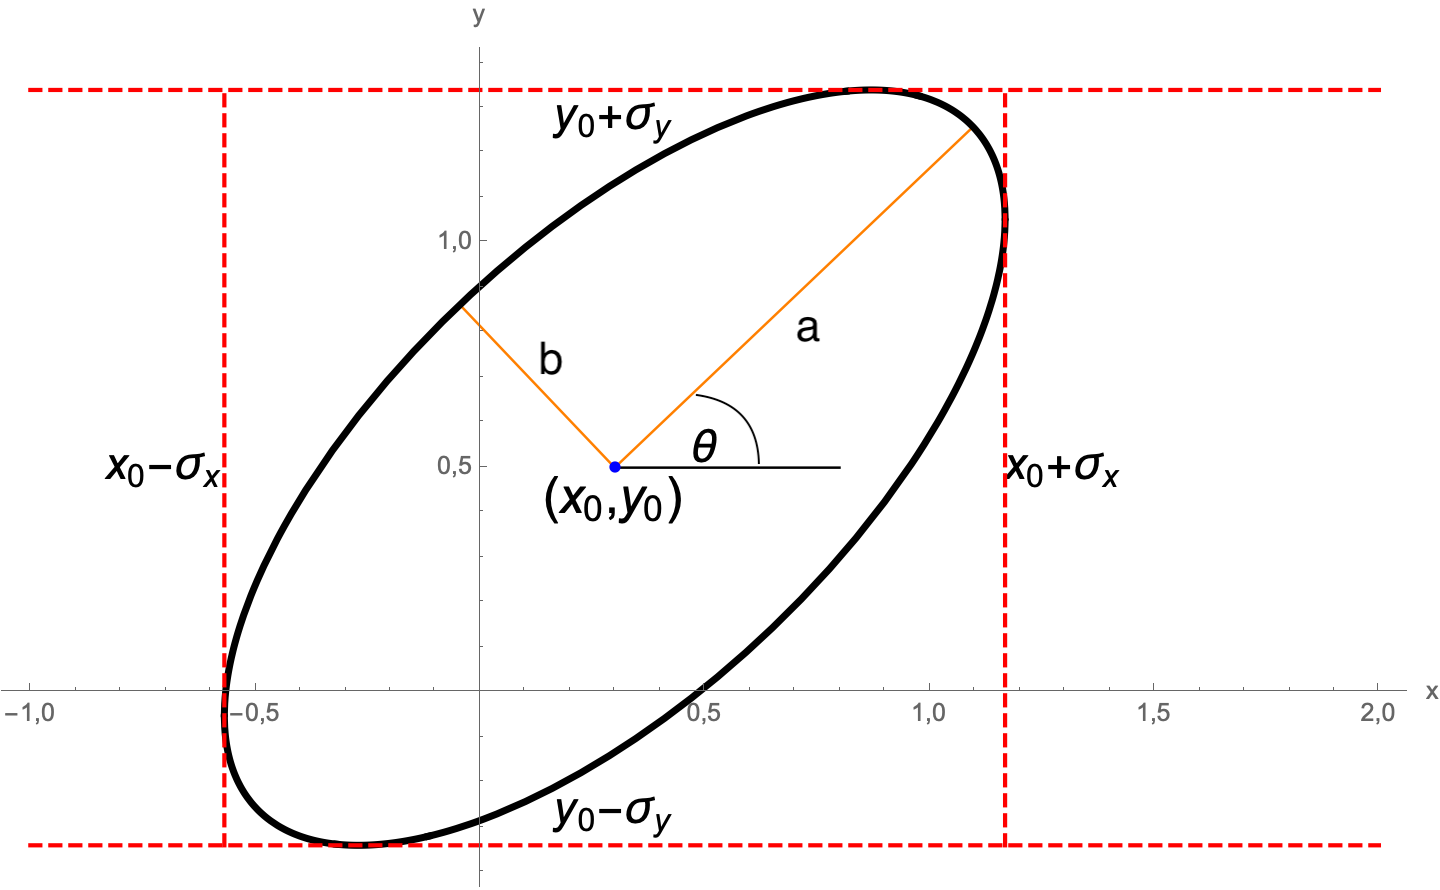
\includegraphics[width=0.6\linewidth]{4-FudgeFactors/2-computationOfUncertainties/ellipse}
%     \caption{Parameters and limits for the most general case of an ellipse.}
%     \label{fig: Computation of FF uncertainties - ellipse}
% \end{figure}

% \begin{figure}[htbp]
%     \centering
%     \includegraphics[width=0.6\linewidth]{4-FudgeFactors/2-computationOfUncertainties/shift_stretch_wtot_et30eta115_ellipse}
%     \caption{Example of an ellipse fit applied to the \(\chi^2 + 2.3\) contour for \(w_{\text{s tot}}\), unconverted photons, \(30~\gev<\pt<40~\gev\) and \(1.15<\abseta<1.37\).}
%     \label{fig: Computation of FF uncertainties - ellipse fit}
% \end{figure}

FIGURE shows the ellipse parameters and limits shown previously, and FIGURE shown an example of application of the fit to the \(w_{\text{s tot}}\) \ac{SS}.
Finally, it is also possible to get the correlation coefficient \(\rho\) as
\begin{equation}
    \rho = \tan(2\theta) \frac{\sigma_{x}^2-\sigma_{y}^2}{2\sigma_{x}\sigma_{y}}.
\end{equation}


\subsection{Systematic uncertainties}

The systematic uncertainties are derived by varying the preselection criteria, that is, photon identification and photon isolation. 
Changing different preselection criteria allows the \acp{SSV} to vary depending on the amount of background contamination, and therefore also the \acp{FF} will change. 
The different selections (also named configurations) are:
\begin{itemize}
    \item \acf{RZ} sample:
        \begin{itemize}
            \item Nominal configuration: No ID, \texttt{FixedCutTightCaloOnly} isolation.
            \item Loose ID, no isolation.
            \item Loose ID, \texttt{FixedCutTightCaloOnly} isolation.
            \item No ID, \texttt{FixedCutLoose} isolation.
        \end{itemize}
    \item \acf{SP} sample:
        \begin{itemize}
            \item Nominal configuration: Tight ID, \texttt{FixedCutLoose} isolation.
            \item Tight ID, \texttt{FixedCutTight} isolation.
        \end{itemize}
\end{itemize}
All other combinations (or lack thereof) of selection criteria would result in either a sample with too low statistics, or too low purity.

\acp{FF} are derived for each one of the previous configurations, and the difference between the ones in the nominal configuration with the remaining ones is calculated. The maximum difference is taken as the systematic uncertainty, as the most conservative approach.












\section{Results}

